\section*{Blatt 1}

\subsection*{1.1 - Scheduling}

Abbildung \ref{fig:fifoScheduler} zeigt die Ausführung von 14 Jobs auf einem System mit 128 Kernen, wobei die Jobs in der Reihenfolge ihrer Ankunft (First-In-First-Out, FIFO) geplant werden. Jeder Job hat eine bestimmte Anzahl von Kernen und eine bestimmte Laufzeit, die durch die Breite und Höhe der Rechtecke dargestellt wird.
Abbildung \ref{fig:easyScheduler} zeigt die gleiche Menge von Jobs, jedoch mit einem "Easy Scheduler", der versucht, die Jobs so zu planen, dass die Ressourcen effizienter genutzt werden. In diesem Fall werden die Jobs so angeordnet, dass sie sich nicht gegenseitig blockieren und die verfügbaren Kerne optimal ausnutzen.

Wir sehen, dass der FIFO-Scheduler zu einer suboptimalen Nutzung der Ressourcen führt, da einige Jobs warten müssen, obwohl genügend Kerne verfügbar sind. Der Easy Scheduler hingegen ermöglicht eine bessere Auslastung der Kerne und reduziert die Wartezeiten für die Jobs.
Anschaulich zu sehen ist dies an der mittleren Verweilzeit\footnote{Die Verweilzeit wird hier definiert als Startzeit minus Ankunftszeit, d.\,h.\ die Wartezeit eines Jobs bis zu seinem Ausführungsbeginn. Diese Definition entstammt dem Modul \textit{Betriebssysteme und Rechnernetze}; in der Vorlesung zu diesem Modul wurde sie leider nicht explizit angegeben.}, die unter dem FIFO-Scheduler mit durchschnittlich 261,43 Einheiten deutlich höher ist als unter dem Easy Scheduler mit durchschnittlich 40,71 Einheiten. Dies zeigt, dass der Easy Scheduler die Jobs effizienter plant und die Ressourcen besser nutzt.

\definecolor{job1color}{RGB}{70,100,230}
\definecolor{job2color}{RGB}{40,140,220}
\definecolor{job3color}{RGB}{20,175,195}
\definecolor{job4color}{RGB}{20,195,155}
\definecolor{job5color}{RGB}{40,205,100}
\definecolor{job6color}{RGB}{90,210,55}
\definecolor{job7color}{RGB}{150,215,40}
\definecolor{job8color}{RGB}{200,210,35}
\definecolor{job9color}{RGB}{225,185,35}
\definecolor{job10color}{RGB}{235,150,40}
\definecolor{job11color}{RGB}{235,110,45}
\definecolor{job12color}{RGB}{225,75,50}
\definecolor{job13color}{RGB}{215,45,55}
\definecolor{job14color}{RGB}{195,25,65}

% \job{x}{y}{width}{height}{color}{label}
\newcommand{\job}[6]{%
  \filldraw[fill=#5, draw=black, line width=0.8pt, rounded corners=4pt]
    (#1,#2) rectangle (#1+#3, #2+#4);
  \node[font=\small\bfseries] at (#1+#3/2, #2+#4/2) {#6};
}

\begin{figure}[H]
  \centering
  \resizebox{\linewidth}{!}{%
  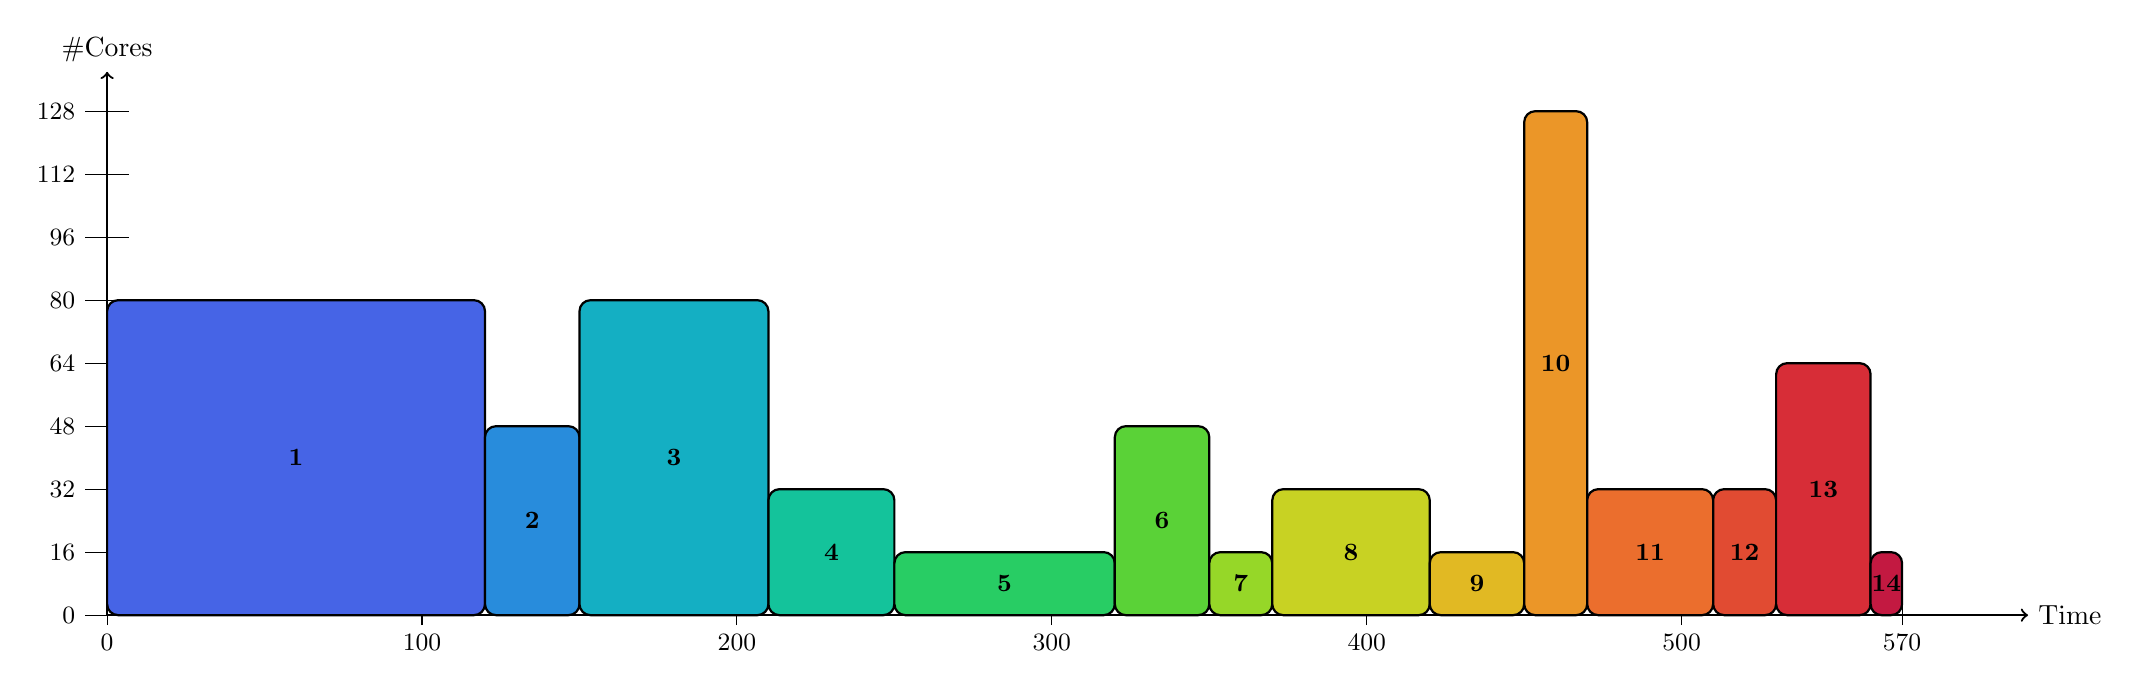
\begin{tikzpicture}[x=0.04cm, y=0.05cm]
    % Axes
    \draw[->, thick] (0,0) -- (610,0) node[right] {Time};
    \draw[->, thick] (0,0) -- (0,138) node[above] {\#Cores};
    % X axis ticks
    \foreach \x in {0,100,200,300,400,500,570} {
      \draw (\x,-2.5) -- (\x,2.5);
      \node[below,font=\small] at (\x,-2.5) {\x};
    }
    % Y axis ticks
    \foreach \y in {0,16,32,48,64,80,96,112,128} {
      \draw (-7,\y) -- (7,\y);
      \node[left,font=\small] at (-7,\y) {\y};
    }
    % Jobs (x, y, width, height, color, label)
    \job{0}{0}{120}{80}{job1color}{1}
    \job{120}{0}{30}{48}{job2color}{2}
    \job{150}{0}{60}{80}{job3color}{3}
    \job{210}{0}{40}{32}{job4color}{4}
    \job{250}{0}{70}{16}{job5color}{5}
    \job{320}{0}{30}{48}{job6color}{6}
    \job{350}{0}{20}{16}{job7color}{7}
    \job{370}{0}{50}{32}{job8color}{8}
    \job{420}{0}{30}{16}{job9color}{9}
    \job{450}{0}{20}{128}{job10color}{10}
    \job{470}{0}{40}{32}{job11color}{11}
    \job{510}{0}{20}{32}{job12color}{12}
    \job{530}{0}{30}{64}{job13color}{13}
    \job{560}{0}{10}{16}{job14color}{14}
  \end{tikzpicture}}
  \caption{Scheduling von Jobs mit einem FIFO-Scheduler}
  \label{fig:fifoScheduler}
\end{figure}

% easy scheduling
\begin{figure}[H]
  \centering
  \resizebox{0.46\linewidth}{!}{%
  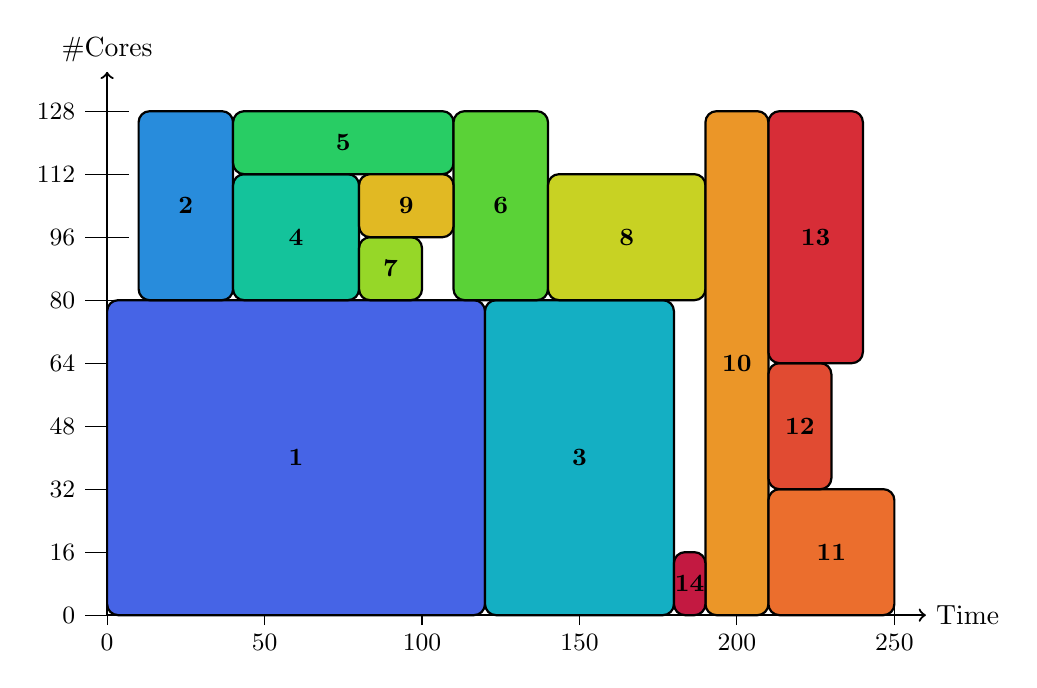
\begin{tikzpicture}[x=0.04cm, y=0.05cm]
    % Axes
    \draw[->, thick] (0,0) -- (260,0) node[right] {Time};
    \draw[->, thick] (0,0) -- (0,138) node[above] {\#Cores};
    % X axis ticks
    \foreach \x in {0,50,100,150,200,250} {
      \draw (\x,-2.5) -- (\x,2.5);
      \node[below,font=\small] at (\x,-2.5) {\x};
    }
    % Y axis ticks
    \foreach \y in {0,16,32,48,64,80,96,112,128} {
      \draw (-7,\y) -- (7,\y);
      \node[left,font=\small] at (-7,\y) {\y};
    }
    % Jobs (x, y, width, height, color, label)
    \job{0}{0}{120}{80}{job1color}{1}
    \job{10}{80}{30}{48}{job2color}{2}
    \job{120}{0}{60}{80}{job3color}{3}
    \job{40}{80}{40}{32}{job4color}{4}
    \job{40}{112}{70}{16}{job5color}{5}
    \job{110}{80}{30}{48}{job6color}{6}
    \job{80}{80}{20}{16}{job7color}{7}
    \job{140}{80}{50}{32}{job8color}{8}
    \job{80}{96}{30}{16}{job9color}{9}
    \job{190}{0}{20}{128}{job10color}{10}
    \job{210}{0}{40}{32}{job11color}{11}
    \job{210}{32}{20}{32}{job12color}{12}
    \job{180}{0}{10}{16}{job14color}{14}
    \job{210}{64}{30}{64}{job13color}{13}
  \end{tikzpicture}}
  \caption{Scheduling von Jobs mit einem Easy Scheduler}
  \label{fig:easyScheduler}
\end{figure}

\begin{table}[H]
  \centering
  \begin{tabular}{|c|r|r|r|r|r|}
    \hline
    \textbf{Job} & \textbf{Ankunft} & \textbf{Startzeit} & \textbf{Laufzeit} & \textbf{Fertigstellung} & \textbf{Verweilzeit} \\
    \hline
    1  &   0 &   0 & 120 & 120 &   0 \\
    2  &  10 & 120 &  30 & 150 & 110 \\
    3  &  20 & 150 &  60 & 210 & 130 \\
    4  &  30 & 210 &  40 & 250 & 180 \\
    5  &  40 & 250 &  70 & 320 & 210 \\
    6  &  50 & 320 &  30 & 350 & 270 \\
    7  &  60 & 350 &  20 & 370 & 290 \\
    8  &  70 & 370 &  50 & 420 & 300 \\
    9  &  80 & 420 &  30 & 450 & 340 \\
    10 & 110 & 450 &  20 & 470 & 340 \\
    11 & 130 & 470 &  40 & 510 & 340 \\
    12 & 140 & 510 &  20 & 530 & 370 \\
    13 & 150 & 530 &  30 & 560 & 380 \\
    14 & 160 & 560 &  10 & 570 & 400 \\
    \hline
    \textbf{Ø} & & & & & \textbf{261,43} \\
    \hline
  \end{tabular}
  \caption{Verweilzeiten unter dem FIFO-Scheduler ($\bar{W} = \tfrac{3660}{14} \approx 261{,}43$)}
  \label{tab:fifoVerweilzeit}
\end{table}

\begin{table}[H]
  \centering
  \begin{tabular}{|c|r|r|r|r|r|}
    \hline
    \textbf{Job} & \textbf{Ankunft} & \textbf{Startzeit} & \textbf{Laufzeit} & \textbf{Fertigstellung} & \textbf{Verweilzeit} \\
    \hline
    1  &   0 &   0 & 120 & 120 &   0 \\
    2  &  10 &  10 &  30 &  40 &   0 \\
    3  &  20 & 120 &  60 & 180 & 100 \\
    4  &  30 &  40 &  40 &  80 &  10 \\
    5  &  40 &  40 &  70 & 110 &   0 \\
    6  &  50 & 110 &  30 & 140 &  60 \\
    7  &  60 &  80 &  20 & 100 &  20 \\
    8  &  70 & 140 &  50 & 190 &  70 \\
    9  &  80 &  80 &  30 & 110 &   0 \\
    10 & 110 & 190 &  20 & 210 &  80 \\
    11 & 130 & 210 &  40 & 250 &  80 \\
    12 & 140 & 210 &  20 & 230 &  70 \\
    13 & 150 & 210 &  30 & 240 &  60 \\
    14 & 160 & 180 &  10 & 190 &  20 \\
    \hline
    \textbf{Ø} & & & & & \textbf{40,71} \\
    \hline
  \end{tabular}
  \caption{Verweilzeiten unter dem Easy Scheduler ($\bar{W} = \tfrac{570}{14} \approx 40{,}71$)}
  \label{tab:easyVerweilzeit}
\end{table}

\subsection*{1.2 - Klassifikation}

\subsection*{Hardwareklassifikation}

Einen einzelnen Knoten können wir als MIMD klassifizieren. Auch schon einer von zwei Prozessoren ist schon in der Lage, mit den 12 Kernen mehrere Instruction Streams und Datastreams zu verarbeiten. Ein zweiter Prozessor ändert die Klassifikation nicht.

Ein verteiltes System mit mehreren Knoten kann gleich Klassifiziert werden. Die Begründung besteht zu einem großen Teil weiter. Allerdings sind die Knoten noch unabhängier voneinander, da sie ganz andere Programme ausführen können. Auf einem einzelnen Knoten wird eine kleinere Menge von Programmen ausgeführt, die dann mehrere Kerne nutzen. Auf einem verteilten System können hingegen mehrere Programme auf verschiedenen Knoten ausgeführt werden, die dann jeweils mehrere Kerne nutzen.

Der Vergleich des einzelnen Knoten mit dem Turing Cluster zeigt schön die in der Vorlesung vorgestellte Unterteilung der Klasse MIMD in jeweils Mehrprozessorsysteme und Verteilte Systeme.

\subsection*{Kommunikationsmodell}

Einzelne Knoten kommunizieren über geteilten Speicher. Da beide Prozessoren integrierte Memory Controller besitzen, können wir den Speicherzugriff als Non-Uniform Memory Access (NUMA)\footnote{\url{https://en.wikipedia.org/wiki/Non-uniform_memory_access}}klassifizieren. So können beide Prozessoren auf den gesamten Hauptspeicher zugreifen, aber die Zugriffszeiten variieren je nachdem, ob der Zugriff auf den lokalen oder den entfernten Speicher erfolgt.

    Verschiedene Knoten kommunizieren über ein Netzwerk, was als Message Passing klassifiziert werden kann. Es gibt keinen gemeinsamen Speicher zwischen den Knoten, und die Kommunikation erfolgt durch den Austausch von Nachrichten über das Netzwerk. Wir können dieses Netzwerk als NORMA einstufen.

\subsection*{1.3 - Netzentwurf}

\subsubsection*{Fat-Tree}

Das entworfene Fat-Tree-Netzwerk besteht aus drei Ebenen, wie in Abbildung~\ref{fig:fatTree} schematisch dargestellt. Da die Uplink-Ports nicht als dedizierte Ports zählen, kann jeder der 64 Leaf-Switches 8 Prozessorkerne anschließen ($512 / 8 = 64$). Diese werden über 8 Switches auf der Zwischenebene verbunden, die wiederum an einen einzelnen Root-Switch angeschlossen sind. Der Durchmesser beträgt 6, da ein Paket maximal 3 Hops zur Wurzel und 3 Hops hinunter zum Ziel benötigt. Blattknoten (Prozessorkerne) haben Grad~1, Intermediate-Switches haben Grad~9 (8 Verbindungen nach unten, 1 nach oben), und der Root-Switch hat Grad~8.

\begin{figure}[H]
  \centering
  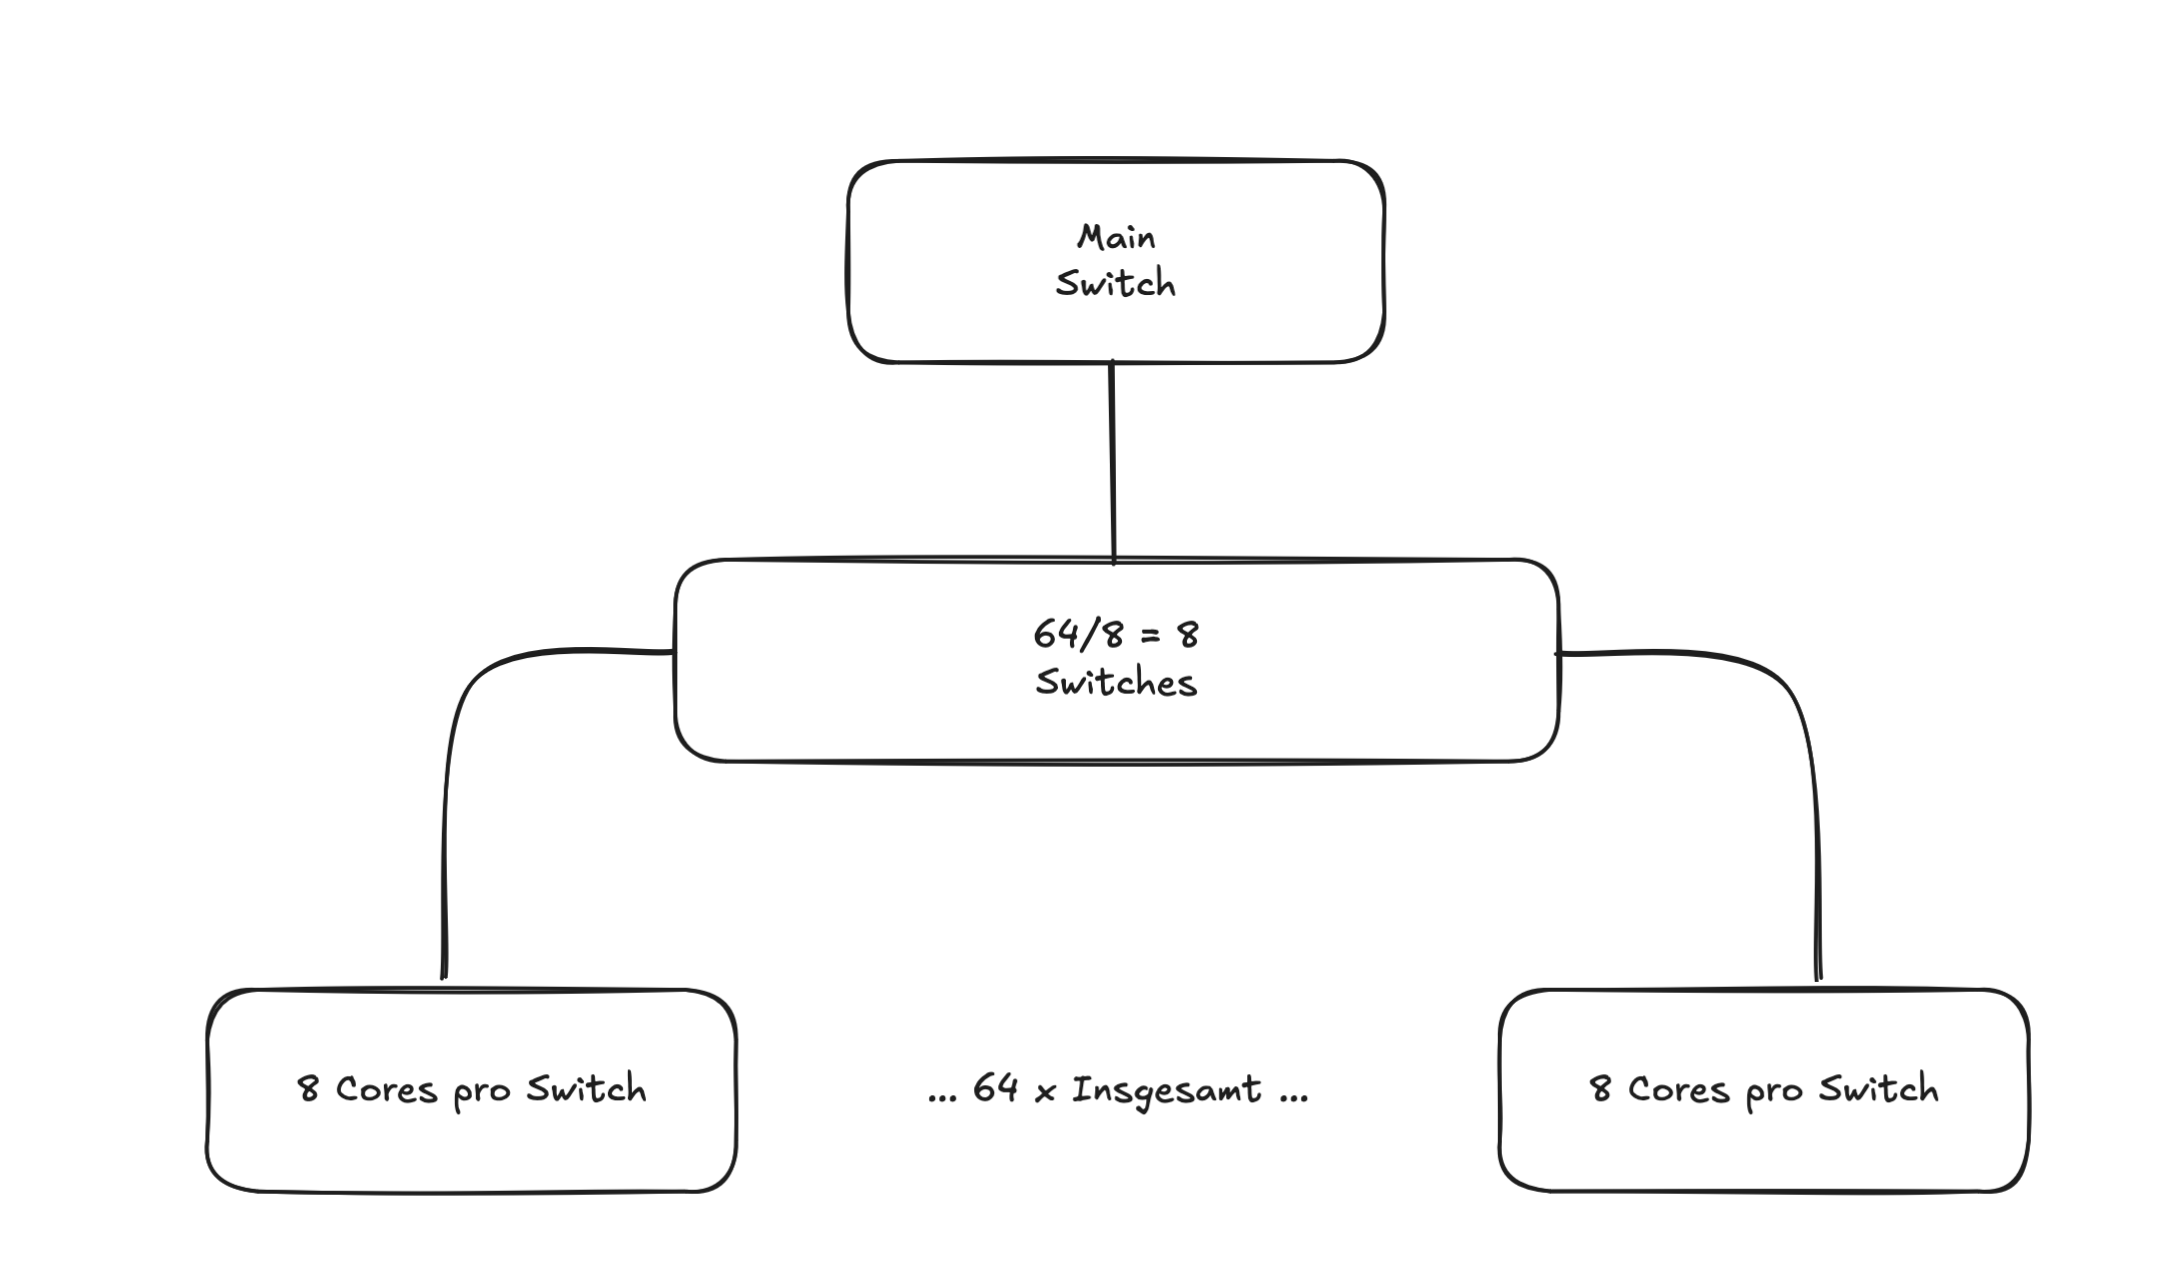
\includegraphics[width=0.8\linewidth]{Images/ex1-3-switches.png}
  \caption{Schematische Darstellung des Fat-Tree-Netzwerks}
  \label{fig:fatTree}
\end{figure}

\subsubsection*{2D-Torus}

Da $\sqrt{512} \notin \mathbb{N}$, wählen wir die Dimensionen $2^4 \times 2^5$.
Der so entstehende Torus ist zwar nicht quadratisch, enthält aber
\[
    2^4 \cdot 2^5 = 2^{4+5} = 2^9 = 512 \text{ Knoten.}
\]
Jeder Knoten hat Grad~4, da er je 2 Verbindungen pro Dimension besitzt. Die
Distanz zwischen zwei Knoten $(x_1, y_1)$ und $(x_2, y_2)$ berechnet sich
dimensionsweise als
\[
    d_{\text{total}} = d(x_1, x_2) + d(y_1, y_2),
\]
wobei die maximale Distanz entlang einer Dimension eines Rings der Länge $m$
gegeben ist durch $\left\lfloor \frac{m}{2} \right\rfloor$. Der Durchmesser
des Torus ergibt sich damit zu:
\[
    d_{\max}
        = \left\lfloor \frac{2^4}{2} \right\rfloor
        + \left\lfloor \frac{2^5}{2} \right\rfloor
        = \left\lfloor \frac{16}{2} \right\rfloor
        + \left\lfloor \frac{32}{2} \right\rfloor
        = 8 + 16 = 24.
\]

\subsubsection*{Vergleich}

\begin{table}[H]
    \centering
    \begin{tabular}{lcc}
        \toprule
        & \textbf{Fat-Tree} & \textbf{2D-Torus ($16 \times 32$)} \\
        \midrule
        Knotengrad  & 1 (Kerne), 8--9 (Switches) & 4 (alle Knoten) \\
        Durchmesser & 6                          & 24              \\
        \bottomrule
    \end{tabular}
    \caption{Vergleich der Netzwerktopologien}
\end{table}

Da Latenz in verteilten Systemen vor allem durch die Anzahl der Hops bestimmt
wird, ist der Fat-Tree klar vorzuziehen: sein Durchmesser von~6 gegenüber~24
beim Torus bedeutet deutlich kürzere Kommunikationswege. Der gleichmäßige
Grad~4 des Torus ist zwar konstruktiv einfacher und hardwaretechnisch
günstiger, rechtfertigt jedoch den sechsfach größeren Durchmesser nicht.

\subsection*{1.4 - Slurm}

\subsubsection*{Aufgabe a}
Ein Ressource Manager (Workload Manager) verwaltet die Ressourcen einer Rechenanlage. Das manuelle Verwalten einer solchen Anlage aufwändig für eine einzelne Person und fast unmöglich für mehrere unabhängig voneinander arbeitende Personen.
Alle müssten sich untereinander abstimmen, damit die Nodes sinnvoll aufgeteilt werden. Zudem müsste auch manuell jeder Job gestartet werden, was jedoch nachts unwahrscheinlich ist.

\subsubsection*{Aufgabe b}
Die \texttt{sbatch} Skripte sind angehängt. Mittels \texttt{make} können diese ausgeführt werden.
